\documentclass{article}
\usepackage[colorlinks=true,linkcolor=blue, citecolor=blue, filecolor=blue, urlcolor=blue]{hyperref}
\usepackage{amsmath}
\usepackage{tikz}
\usetikzlibrary{shapes.geometric,shapes.arrows,decorations.pathmorphing,
decorations.markings,decorations.pathreplacing}
\usetikzlibrary{matrix,chains,scopes,positioning,arrows,fit,spy,calligraphy}

\begin{document}

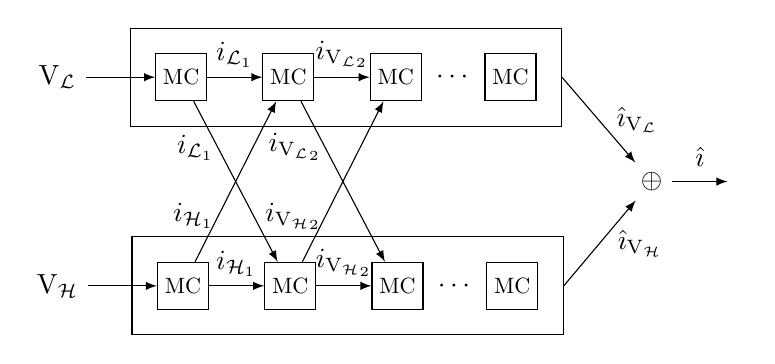
\begin{tikzpicture}[auto, node distance=2cm, >=latex]
\tikzstyle{block} = [draw, minimum height=0.75cm, minimum width=0.8cm, scale=0.8]
\tikzstyle{wrapper} = [draw, minimum height=0.75cm, minimum width=0.8cm, inner sep=9pt]

\node (low_vis) at (0, 0) [above=10pt]{$\text{V}_\mathcal{L}$};

\node (mc1l) at (low_vis.east) [block, right=25pt] {MC};
\node (mc2l) at (mc1l.east) [block, right=20pt] {MC};
\node (mc3l) at (mc2l.east) [block, right=20pt] {MC};
\node (low_ell) at (mc3l.east) [minimum height=0.75cm, minimum width=0.75cm, right=1pt] {$\cdots$};
\node (mcnl) at (low_ell.east) [block, right=0pt] {MC};

\draw [->] (low_vis) edge (mc1l);
\draw [->] (mc1l) -- node [midway, above=0pt] {$i_{\mathcal{L}_1}$} (mc2l); 
\draw [->] (mc2l) -- node [midway, above=0pt] {$i_{{\text{V}_\mathcal{L}}_2}$} (mc3l); 

\node[fit=(mc1l)(mc2l)(mcnl), wrapper](vlnode){};

\node (full_vis) at (low_vis.south)[below=60pt]{$\text{V}_\mathcal{H}$};

\node (mc1h) at (full_vis.east) [block, right=25pt] {MC};
\node (mc2h) at (mc1h.east) [block, right=20pt] {MC};
\node (mc3h) at (mc2h.east) [block, right=20pt] {MC};
\node (low_ell) at (mc3h.east) [minimum height=0.75cm, minimum width=0.75cm, right=1pt] {$\cdots$};
\node (mcnh) at (low_ell.east) [block, right=0pt] {MC};

\draw [->] (full_vis) edge (mc1h);
\draw [->] (mc1h) -- node [midway, above=0pt] {$i_{\mathcal{H}_1}$} (mc2h); 
\draw [->] (mc2h) -- node [midway, above=0pt] {$i_{{\text{V}_\mathcal{H}}_2}$} (mc3h); 

\draw [->] (mc1h) -- node [midway, below left=6pt] {$i_{\mathcal{H}_1}$} (mc2l); 
\draw [->] (mc2h) -- node [midway, below left=6pt] {$i_{{\text{V}_\mathcal{H}}_2}$} (mc3l); 
\draw [->] (mc1l) -- node [midway, above left=6pt] {$i_{\mathcal{L}_1}$} (mc2h); 
\draw [->] (mc2l) -- node [midway, above left=6pt] {$i_{{\text{V}_\mathcal{L}}_2}$} (mc3h); 

\node[fit=(mc1h)(mc2h)(mcnh), wrapper](vhnode){};

\node[fit=(mcnl)(mcnh)](centeringnode){};
\node (comb) at (centeringnode.east)[right=30pt]{$\oplus$};
\node (dummyout) at (comb.east)[right=20pt]{};

\draw [->] (vlnode.east) -- node [midway, right=3pt] {$\hat{\imath}_{\text{V}_\mathcal{L}}$} (comb); 
\draw [->] (vhnode.east) -- node [midway, right=3pt] {$\hat{\imath}_{\text{V}_\mathcal{H}}$} (comb); 
\draw [->] (comb) -- node [midway, above=2pt] {$\hat{\imath}$} (dummyout); 

\end{tikzpicture}

\end{document}